\documentclass[]{rsuqbeamernew}


\title[]{Distributed computing in UQLab\\with the HPC Dispatcher module}

\author[D. Wicaksono]{Damar Wicaksono}
\institute[RSUQ, ETH Z\"urich]{Chair of Risk, Safety and Uncertainty 
Quantification -- ETH Z\"urich}

\date[09.05.2019]

\graphicspath{{Figures/}}
\usepackage{caption}
\usepackage{listings}
\usepackage{tikz}
\usepackage{pifont}
\usepackage{booktabs}% http://ctan.org/pkg/booktabs
\usepackage{xcolor}
\definecolor{myviolet}{RGB}{140,92,180}
\newcommand{\tabitem}{~~\llap{\textbullet}~~}
%\def\checkmark{\tikz\fill[scale=0.4](0,.35) -- (.25,0) -- (1,.7) -- (.25,.15) -- cycle;}

\lstset{
  basicstyle=\ttfamily,
  escapeinside=||
}

\definecolor{codegreen}{rgb}{0,0.6,0}
\definecolor{codegray}{rgb}{0.5,0.5,0.5}
\definecolor{codepurple}{rgb}{0.58,0,0.82}
\definecolor{backcolour}{rgb}{0.95,0.95,0.92}

\lstdefinestyle{mystyle}{
    backgroundcolor=\color{backcolour},   
    commentstyle=\color{codegreen},
    keywordstyle=\color{magenta},
    numberstyle=\tiny\color{codegray},
    stringstyle=\color{codepurple},
    basicstyle=\ttfamily\footnotesize,
    breakatwhitespace=false,         
    breaklines=true,                 
    captionpos=b,                    
    keepspaces=true,                 
    numbers=left,                    
    numbersep=5pt,                  
    showspaces=false,                
    showstringspaces=false,
    showtabs=false,                  
    tabsize=2
}

\lstset{style=mystyle}


%% Note: the title page will be created automatically

\newsavebox{\mysavebox}

\begin{document}

%%%%%%%%%%%%%%%%%%%%
\section{Motivation}
%%%%%%%%%%%%%%%%%%%%

%===============================================================================
\begin{frame}{Background}

\begin{block}{Some problems \textsc{UQLab} users might have:}
\begin{itemize}
  \item They need to run long-running computation; they only have their laptops\\
        \onslide<2>{\textcolor{myviolet}{$\rightarrow$ freeing up local computing resources}}
  \item They need to run computations with large memory or CPU requirements\\
        \onslide<2>{\textcolor{myviolet}{$\rightarrow$ exceptional resources (CPU, memory) requirement}}
  \item Their simulation code only runs in Linux with, possibly, special licensing
        \onslide<2>{\textcolor{myviolet}{$\rightarrow$ compatibility and licensing issues}}
\end{itemize}
\end{block}

\end{frame}

%==============================================================================
\begin{frame}
\frametitle{Background}

\begin{block}{Distributed computing resources might help:}
\begin{itemize}
  \item They are highly available round the clock
        \onslide<2>{(\textcolor{myviolet}{\textbf{not always}})}
  \item They have massive amount of high-performance CPUs, memory, and storage
        \onslide<2>{(\textcolor{myviolet}{\textbf{not always}})}
  \item They come with expensive software installed with shared licenses
        \onslide<2>{(\textcolor{myviolet}{\textbf{not always}})}
\end{itemize}
\end{block}

\begin{onslide}<2>
\begin{block}{Distributed computing resources come in many forms and flavors}
  \begin{columns}
    \begin{column}{.3\linewidth}\centering
    \includegraphics<2>[width=0.65\linewidth]{Beowulf}\\
    \only<2>{{\tiny Credit: Wikipedia, GPL v3}}
    \end{column}
    \begin{column}{.3\linewidth}\centering
    \includegraphics<2>[width=\linewidth]{blue-gene}\\ 
    \only<2>{{\tiny Credit:Argonne National Lab.,CC BY-SA2.0}}
    \end{column}
    \begin{column}{.3\linewidth}\centering
    \includegraphics<2>[width=0.75\linewidth]{blue-paper-with-clouds}\\
    \only<2>{{\tiny Credit: Zamurovic Brothers (Noun Project)}}
    \end{column}
    \end{columns}
\end{block}
\end{onslide}

\end{frame}

%==============================================================================
\begin{frame}
\frametitle<1>{Distributed computing resources might help}
\frametitle<2>{Distributed computing resources might help, but...}

\begin{block}{Your institution provides distributed computing resources, so you:}
\begin{enumerate}
  \item ask or look around how to get an access
  \item get an access (username, password, computing time, storage space)
  \item read the Wiki
  \item are ready for some distributed computing \only<2>{{\altx (right?)}}
\end{enumerate}
\end{block}

\begin{block}{\textbf{EULER}: The large HPC infrastructure of the ETHZ}
\begin{figure}[htbp]
  \includegraphics[width=\textwidth]{./figures/ETH_Zurich_Euler_II_and_I_in_LCA}\\
  {\tiny Credit: Olivier Byrde, ETH Zurich (2015)}
\end{figure}
\end{block}

\end{frame}

%==============================================================================
\begin{frame}
\frametitle<1-7>{Distributed computing in 7 easy steps}
\frametitle<8>{Distributed computing in 7 (\emph{not so}) easy steps}
\begin{columns}
\column{0.4\textwidth}
\setbeamercovered{invisible}
\begin{block}{The steps:}
\begin{enumerate}
  \item<2-> Log in to the remote machine
  \item<3-> Create an analysis script to run in the remote
  \item<4-> Create a job script
  \item<5-> Submit the job to the queues
  \item<6-> Check the queues until job is finished
  \item<7-> Transfer output files back (\texttt{scp}, \texttt{rsync})
  \item<8-> Analyze the outputs in the local machine
\end{enumerate}
\end{block}
\column{0.6\textwidth}
\begin{onlyenv}<2-8>
\begin{figure}[htbp]
  \includegraphics<2>[width=\textwidth]{./figures/terminal-small.png}
  \includegraphics<3>[width=\textwidth]{./figures/remote-script.png}
  \includegraphics<4>[width=\textwidth]{./figures/job-script.png}
  \includegraphics<5>[width=\textwidth]{./figures/queues.png}
  \includegraphics<6>[width=\textwidth]{./figures/check-queues.png}
  \includegraphics<7>[width=\textwidth]{./figures/scp.png}
  \includegraphics<8>[width=\textwidth]{./figures/matlab.png}
\end{figure}
\end{onlyenv}
\setbeamercovered{transparent}
\end{columns}
\end{frame}

%==============================================================================
\begin{frame}
\frametitle{Users vs. Machine}
\begin{figure}[htbp]
  \includegraphics[width=0.9\textwidth]{./figures/dispatcher-gap.pdf}
\end{figure}

\begin{columns}
  \begin{column}{0.5\linewidth}
    \begin{block}{Users are used to:}
      \begin{itemize}
        \item {\altx synchronous execution}: immediate execution
        \item {\altx local storage}: results are available on completion
        \item {\altx think of a serial program}: easier to debug
      \end{itemize}
    \end{block}
  \end{column}
  \begin{column}{0.5\linewidth}
    \begin{block}{Now, users have to get used to:}
      \begin{itemize}
        \item {\altx asynchronous execution}: schedule and submit an execution
        \item {\altx remote storage}: results must be retrieved
        \item {\altx think of parallel program}: harder to debug (e.g., race conditions)
      \end{itemize}
    \end{block}
  \end{column}
\end{columns}

\end{frame}
  
%==============================================================================
\begin{frame}
\frametitle{Introducing the HPC \textsc{Dispatcher} module}

\begin{figure}[htbp]
  \includegraphics[width=0.95\textwidth]{./figures/dispatcher-module.pdf}
\end{figure}    

\begin{onlyenv}<1>
\begin{block}{The HPC \textsc{dispatcher} module is an attempt to bridge the gap}
  \begin{itemize}
    \item It allows user to dispatch and retrieve {\altx some computations}
          to remote distributed computing resources
    \item All from a local \textsc{UQLab} session
    \item Emphasis on {\altx some computations}, i.e.,
          certain computations that are relevant in uncertainty quantification (UQ)
          with \textsc{UQLab}
  \end{itemize}
\end{block}
\end{onlyenv}

\setbeamercovered{invisible}
\begin{onlyenv}<2-3>
  \begin{onslide}<2->
  \begin{block}{This presentation is about:}
    \begin{itemize}
      \item The HPC \textsc{dispatcher} module features
      \item Its basic usage and a couple of more advanced use cases
    \end{itemize}
  \end{block}
\end{onslide}

\begin{onslide}<3->
  \begin{block}{...and less about (if at all):}
    \begin{itemize}
      \item Distributed computing system and organization
      \item Parallel algorithms and programming
    \end{itemize}
  \end{block}
\end{onslide}
\end{onlyenv}
\setbeamercovered{transparent}

\end{frame}

\begin{frame}[fragile]{Introducing the HPC \textsc{Dispatcher} module}

Watch this slide grow.
\pause
\begin{itemize}
  \item<2-> Hello, World!
  \item<3-> Hello, Mars!
  \item<4-> \textbf<5->{Hello}, Alpha Centauri!
\end{itemize}
  
\end{frame}

\begin{frame}[fragile]{\texttt{uq\_map}: Mapping function}

\begin{lstlisting}
uq_map(|\textcolor<2>{myviolet}{fun}|,|\textcolor<3>{myviolet}{inputs}|)
\end{lstlisting}
\begin{itemize}
  \item \textcolor<2>{myviolet}{mapping function}
  \item \textcolor<3>{myviolet}{input sequence}
\end{itemize}

\end{frame}

%%%%%%%%%%%%%%%%%%%%%%%%%%%%%%%%%%%%%%%
\section{\textsc{Dispatcher} in action}
%%%%%%%%%%%%%%%%%%%%%%%%%%%%%%%%%%%%%%%

%==============================================================================
\begin{frame}[fragile]
\frametitle<1>{\textsc{Dispatcher} in action: Problem setup}
\frametitle<2->{\textsc{Dispatcher} in action: \textsc{Model} evaluation}

Create a \textsc{Model} object from an \mcode{m}-file:
\begin{lstlisting}[basicstyle=\scriptsize]
ModelOpts.mFile = 'uq_ishigami';

myModel = uq_createModel(ModelOpts);
\end{lstlisting}

\begin{onlyenv}<2-2>
Evaluate the \textsc{Model} on a single input point:
\begin{lstlisting}[basicstyle=\scriptsize,numbers=none]
>> uq_evalModel([0.5*pi 0.5*pi 0.5*pi])

ans =
  
    8.6088
\end{lstlisting}
\end{onlyenv}

\begin{onlyenv}<3->
Let's assume a \textsc{Dispatcher} object has been created
and stored in a variable \mcode{myDispatcher} ({\altx more on this later}).
Dispatch the same \textsc{Model} evaluation to the remote machine:
\begin{lstlisting}[basicstyle=\scriptsize,numbers=none]
>> uq_evalModel([0.5*pi 0.5*pi 0.5*pi],'HPC')
  
ans =
    
    []
\end{lstlisting}
\end{onlyenv}

\setbeamercovered{invisible}
\onslide<4->{\emphconc{Whoa, what happened?}}
\setbeamercovered{transparent}
  
\end{frame}

%==============================================================================
\begin{frame}[fragile]{\textsc{Dispatcher} in action: \emph{Dispatch} a computation}

\begin{lstlisting}[basicstyle=\scriptsize,numbers=none]
>> uq_evalModel(myModel, X, 'HPC')
  
ans =
  
    []
\end{lstlisting}
  
\begin{figure}[htbp]    
  \centering
  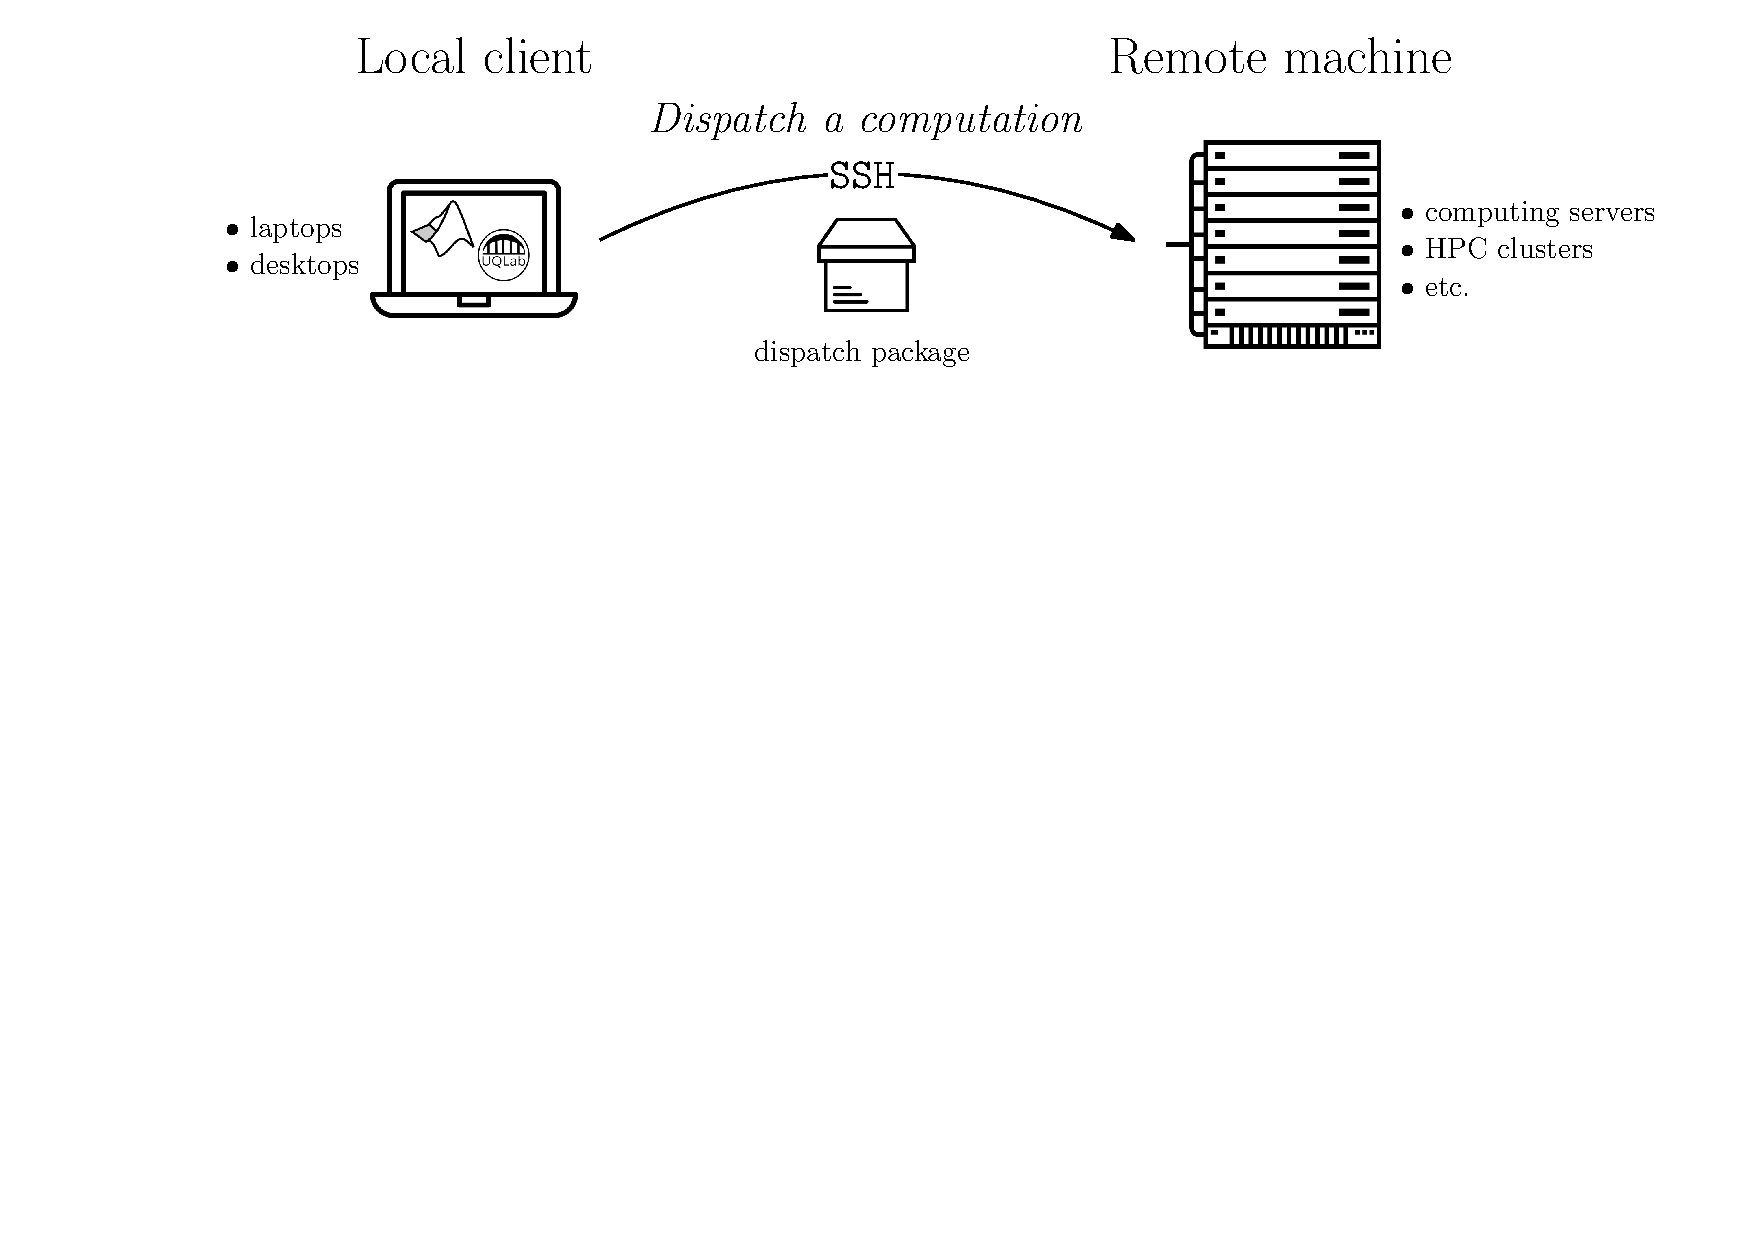
\includegraphics[width= 0.8\textwidth]{./figures/dispatch-and-fetch-dispatch.pdf}
\end{figure}

\end{frame}

%==============================================================================
\begin{frame}[fragile]{Dispatcher in action: asynchronous execution}

\begin{lstlisting}[basicstyle=\scriptsize,numbers=none]
>> uq_evalModel(myModel,X,'HPC')
    
ans =

    []
\end{lstlisting}
    
\begin{figure}[htbp]    
  \centering
  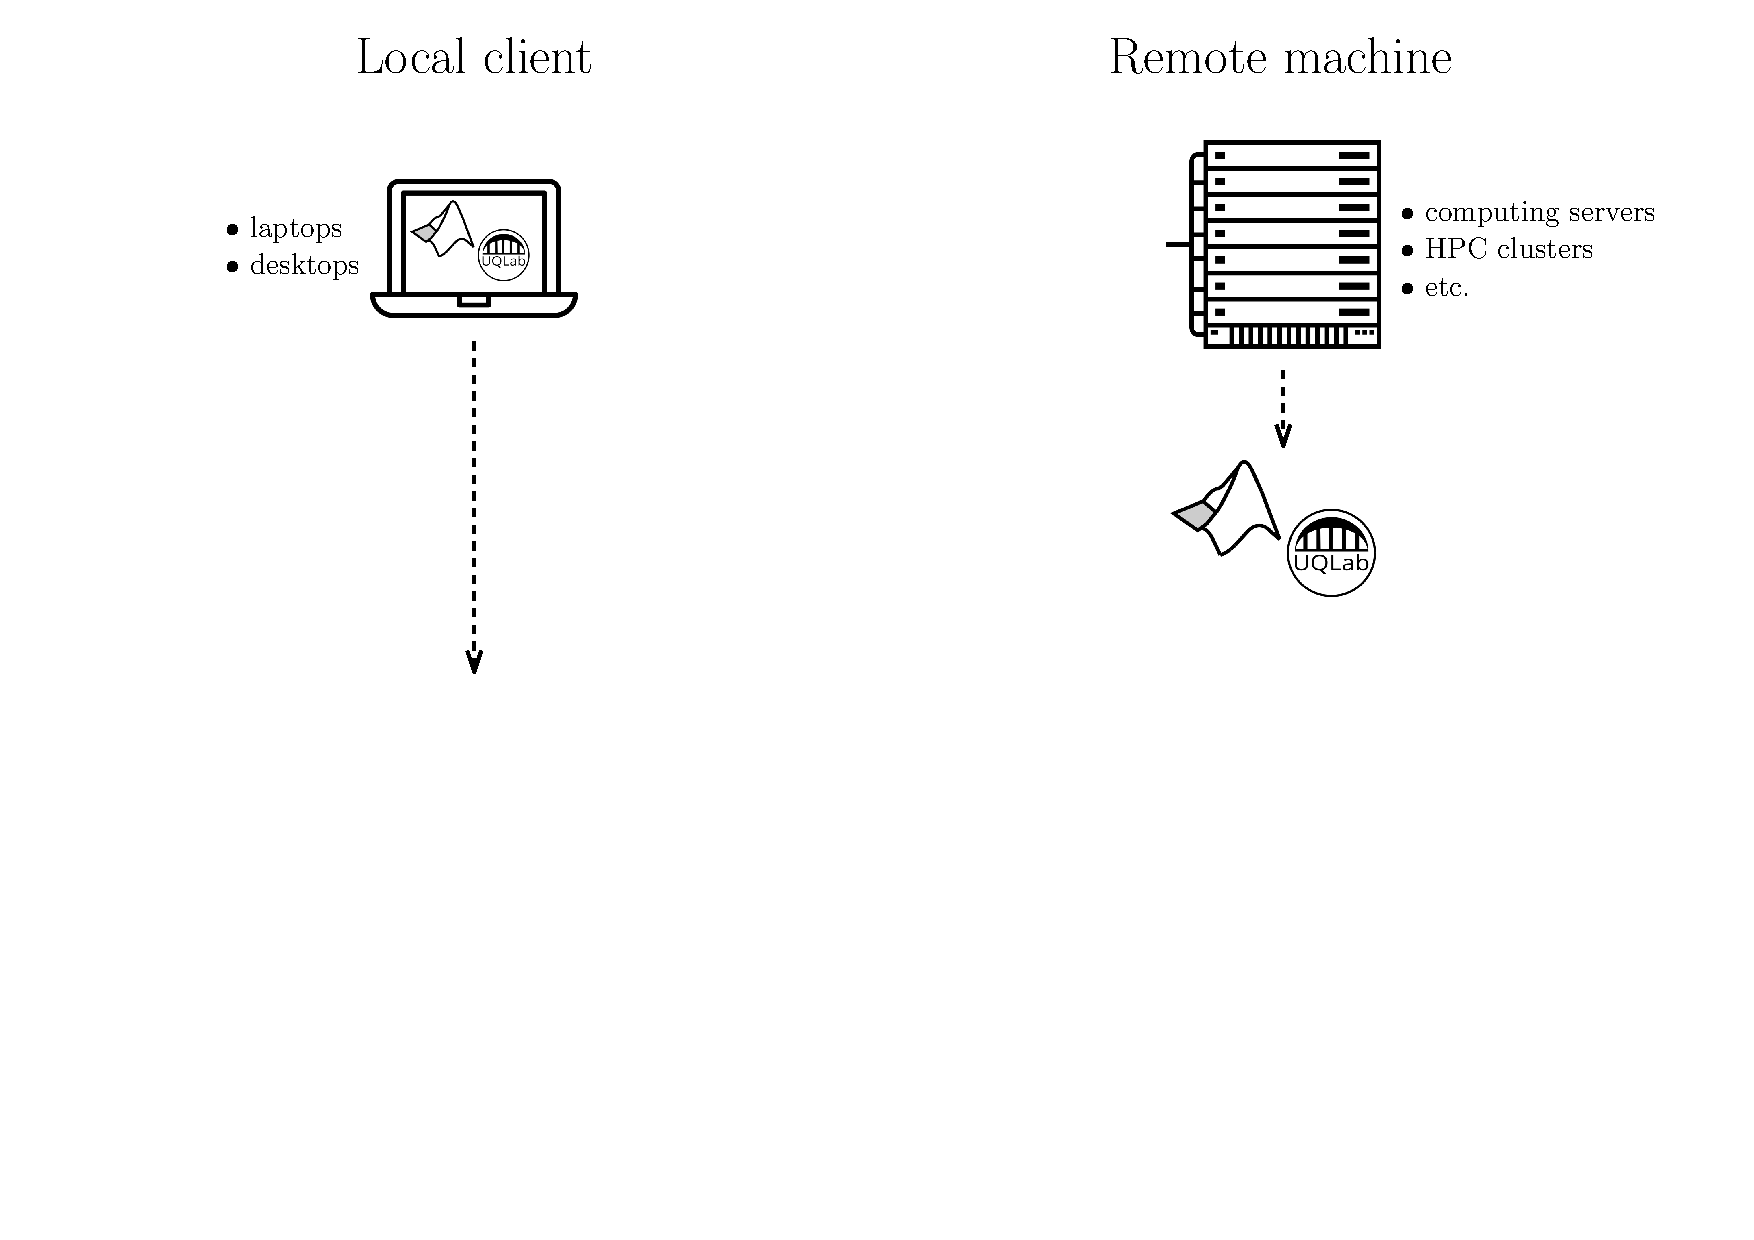
\includegraphics[width= 0.8\textwidth]{./figures/dispatch-and-fetch-asynchronous.pdf}
\end{figure}
  
\end{frame}

%==============================================================================
\begin{frame}[fragile]{Dispatcher in action: \emph{Get status}}

\begin{lstlisting}[basicstyle=\scriptsize,numbers=none]
>> uq_getStatus(myDispatcher)
      
ans =

    'running'
\end{lstlisting}
      
\begin{figure}[htbp]    
  \centering
  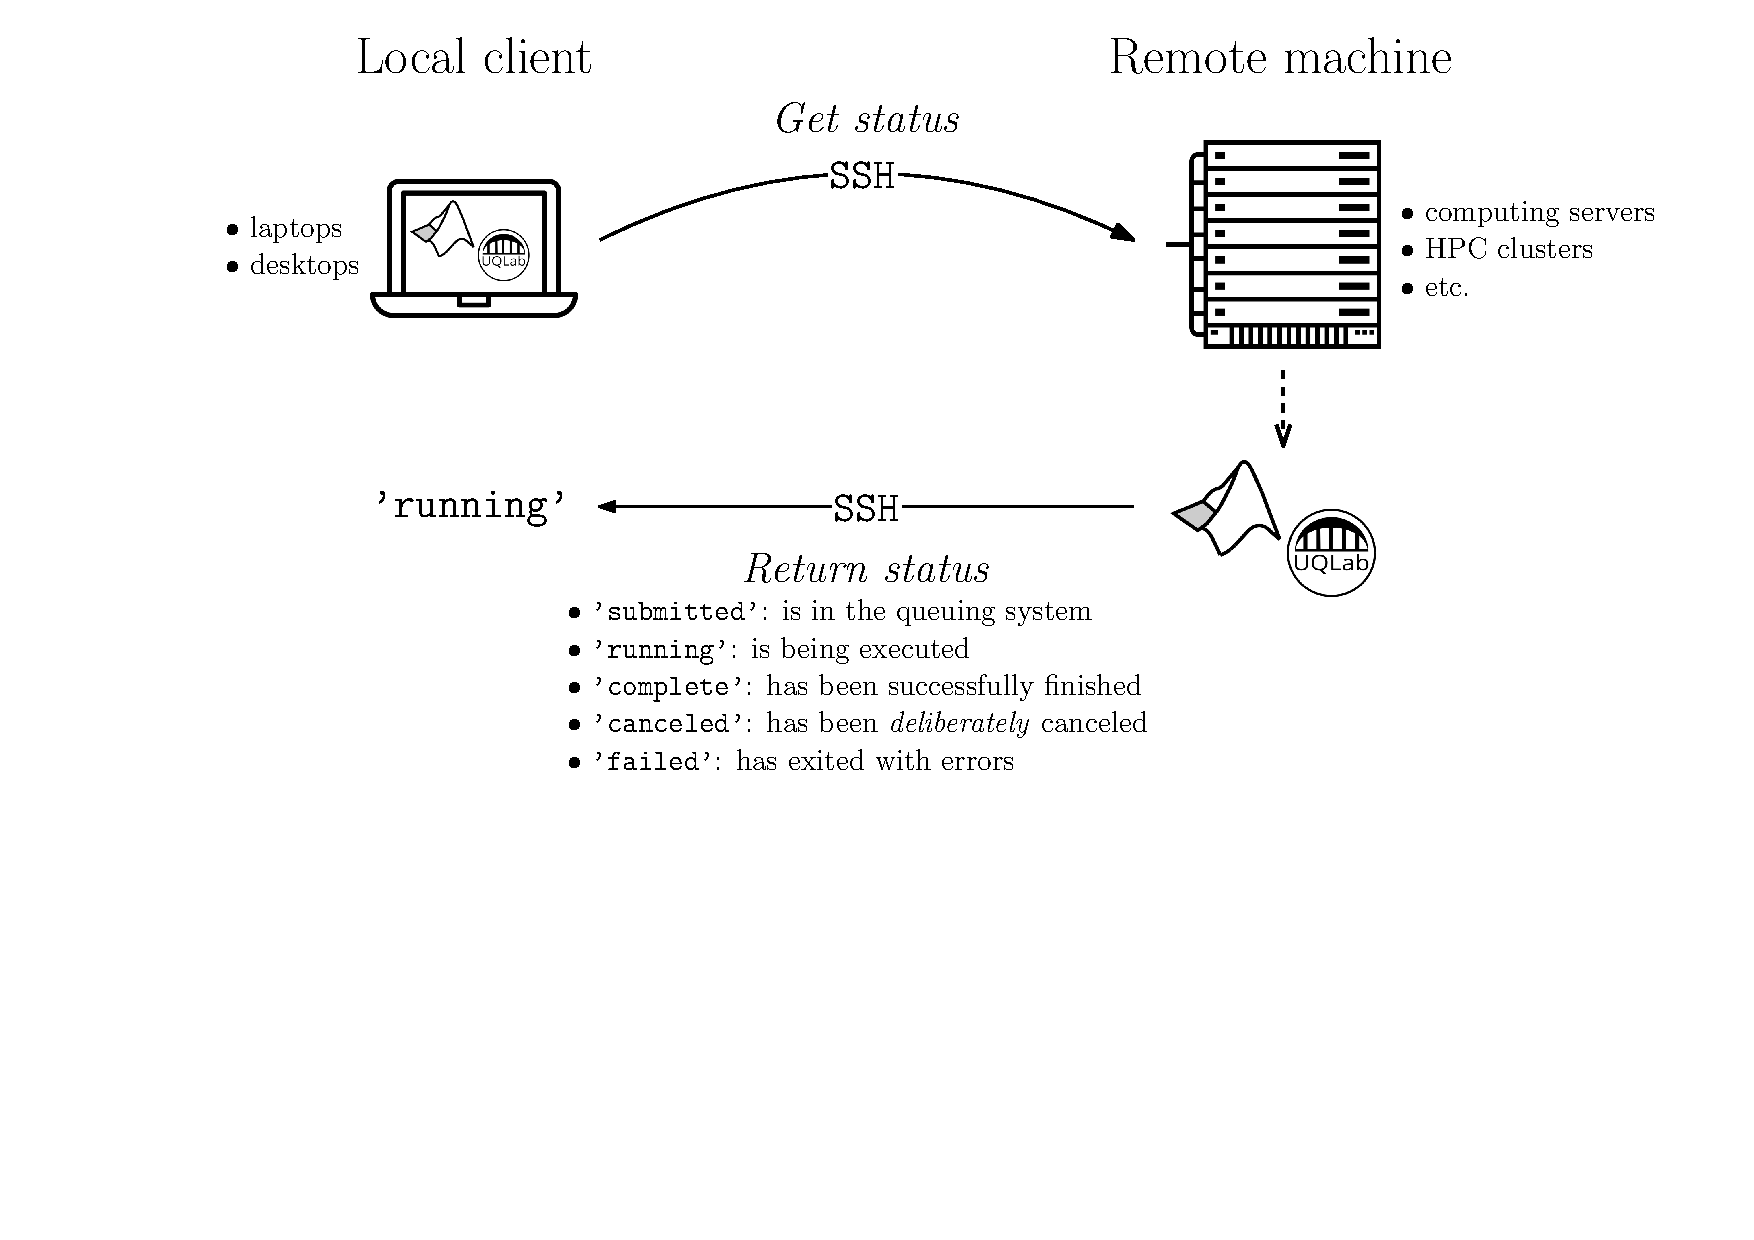
\includegraphics[width= 0.8\textwidth]{./figures/dispatch-and-fetch-getStatus.pdf}
\end{figure}
    
\end{frame}

%==============================================================================
\begin{frame}[fragile]{Dispatcher in action: remote execution is finished}

\begin{lstlisting}[basicstyle=\scriptsize,numbers=none]
>> uq_getStatus(myDispatcher)
      
ans =
  
  'complete'
\end{lstlisting}
      
\begin{figure}[htbp]    
  \centering
  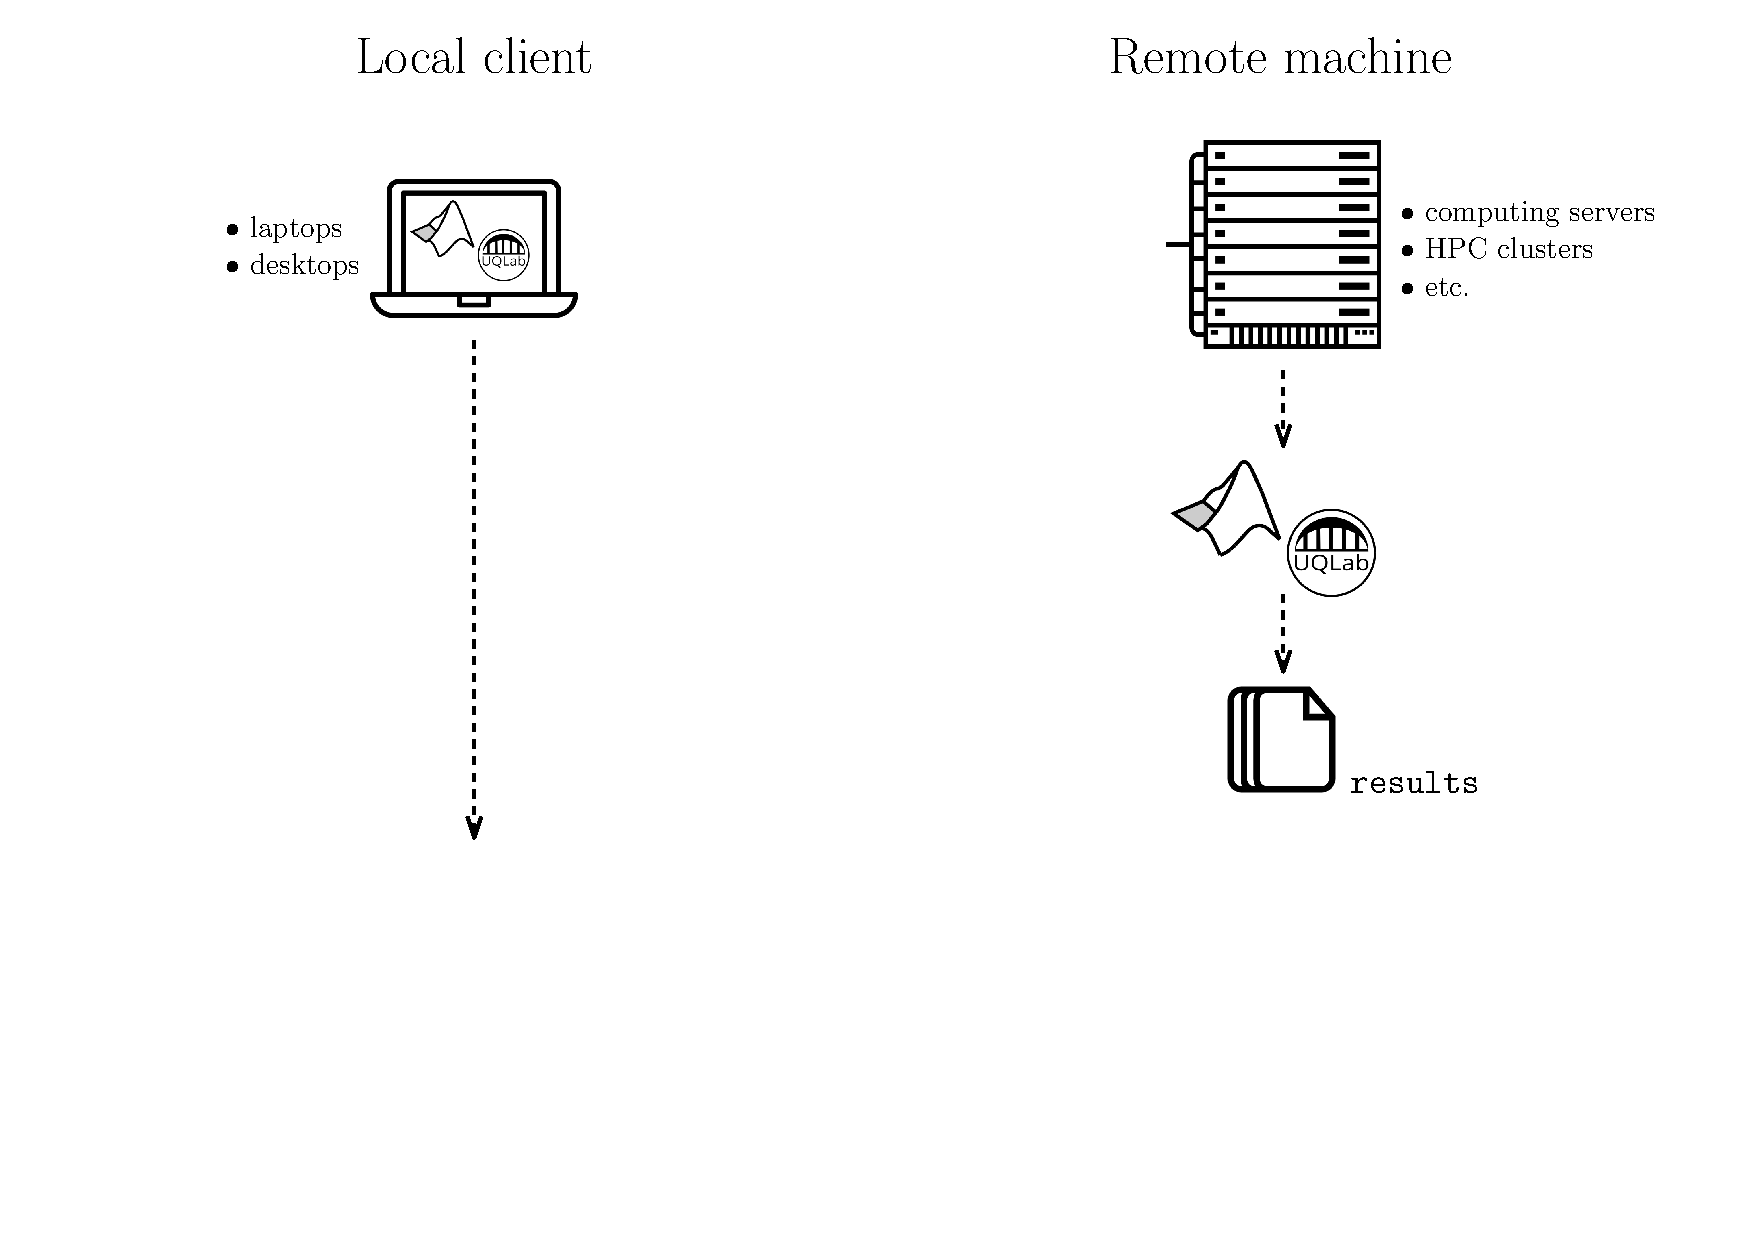
\includegraphics[width= 0.8\textwidth]{./figures/dispatch-and-fetch-completed.pdf}
\end{figure}
    
\end{frame}

%==============================================================================
\begin{frame}[fragile]{Dispatcher in action: \emph{Fetch} the results}

\begin{lstlisting}[basicstyle=\scriptsize,numbers=none]
>> results = uq_fetchResults(myDispatcher)

results =

    8.6088
\end{lstlisting}
        
\begin{figure}[htbp]
  \centering
  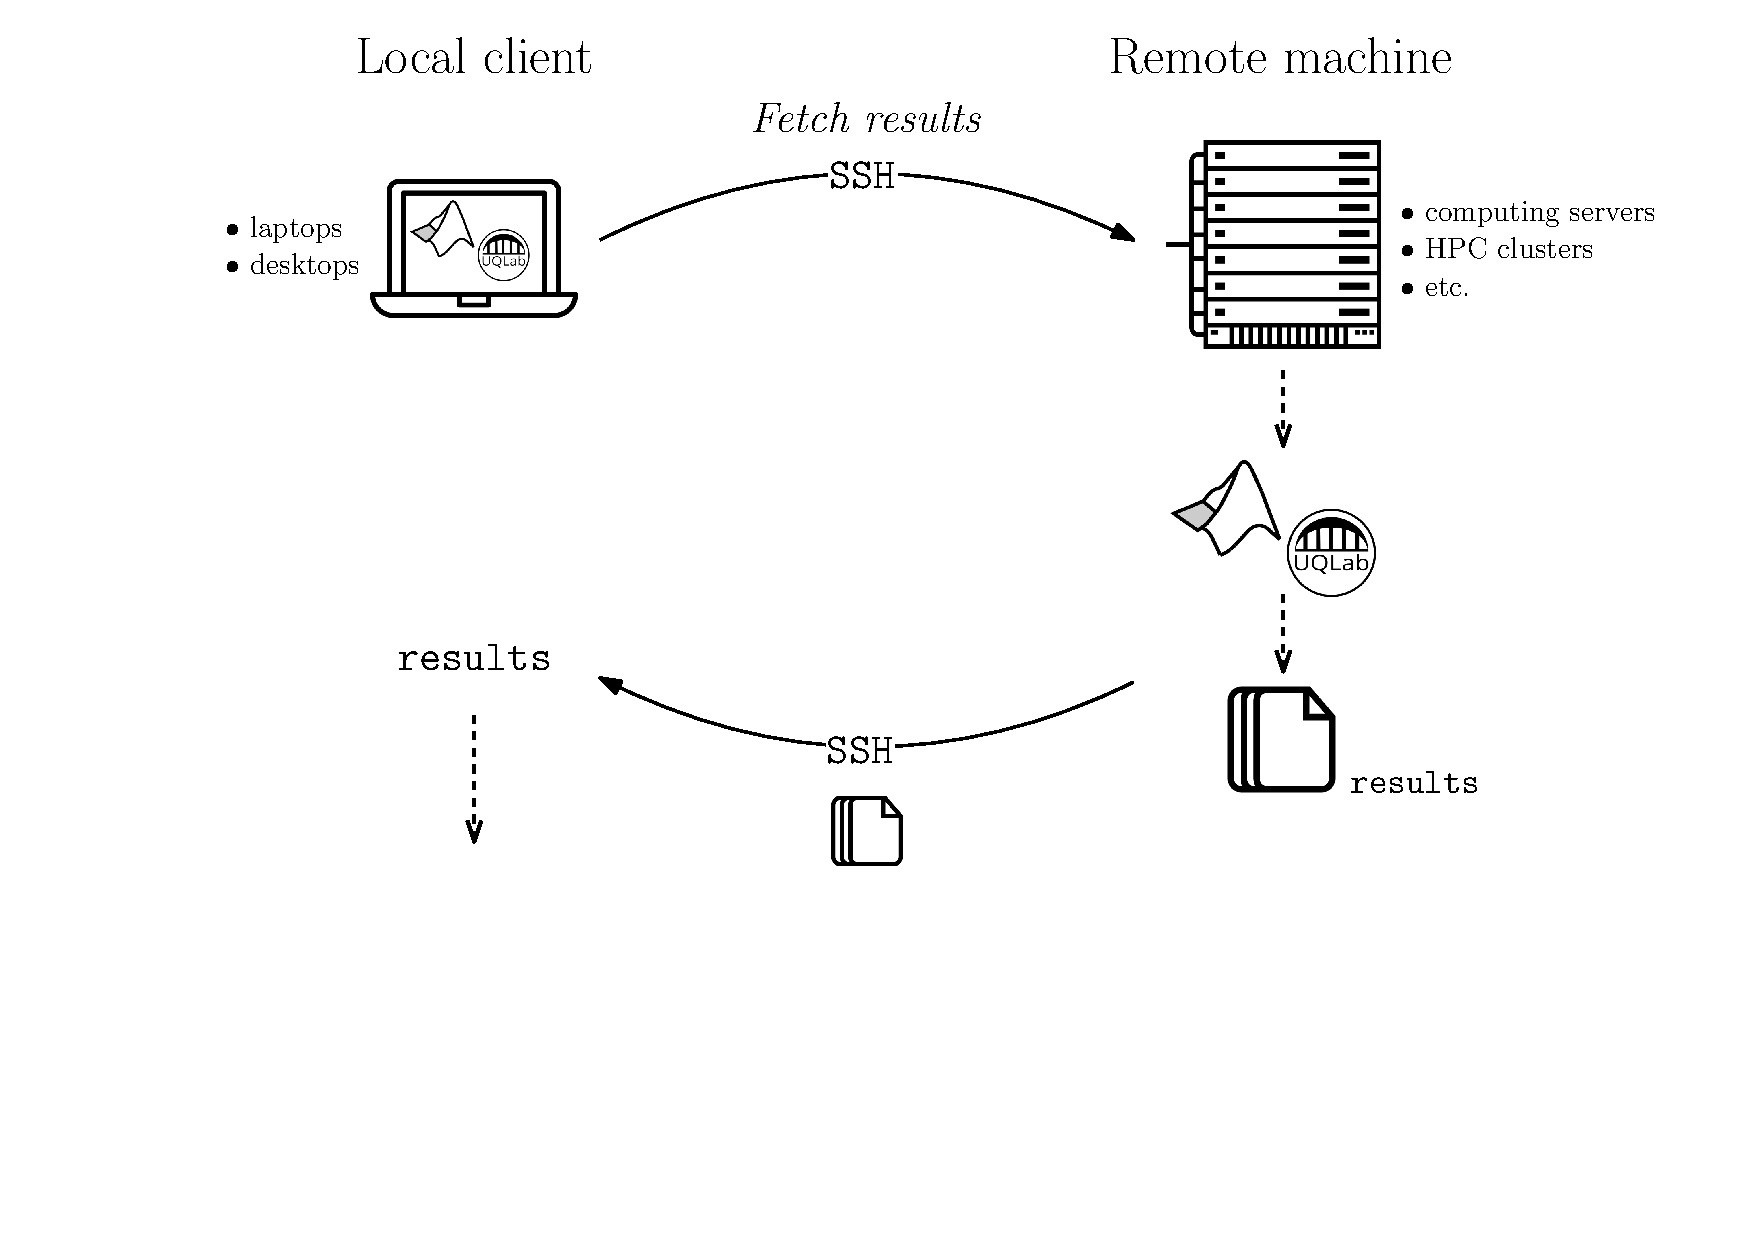
\includegraphics[width= 0.8\textwidth]{./figures/dispatch-and-fetch-fetchResults.pdf}
\end{figure}
      
\end{frame}

%==============================================================================
\begin{frame}[fragile]{Backtracking: Setting up a Dispatcher object}

\only<1-3>{\begin{block}{What you need to set up and use a \textsc{Dispatcher} object}
\begin{itemize}
  \item An access to a remote machine; it must run a Linux OS and has an MPI implementation
  \item A directory with write access permission in the remote machine
  \item A passwordless SSH connection to the remote machine
  \item A profile file that stores required information about the remote machine 
\end{itemize}
\end{block}}

\only<4>{\emphconc{No \textsc{MATLAB}/\textsc{UQLab} in the remote machine is required
for \textsc{UQLink} model evaluation}}

\begin{onslide}<2->
An example of a (minimum) remote machine profile file (\texttt{myProfile.m}):
\begin{lstlisting}[basicstyle=\scriptsize]
Hostname = 'euler.ethz.ch';
Username = 'wdamar';
PrivateKey = '~/.ssh/id_rsa_dispatcher';
RemoteFolder = '/home/wdamar/temp';
\end{lstlisting}
\end{onslide}

\begin{onslide}<3->
In a \textsc{UQLab} session:
\begin{lstlisting}[basicstyle=\scriptsize,numbers=none]
DispatcherOpts.Profile = 'myProfile';
  
myDispatcher = uq_createDispatcher(DispatcherOpts);
\end{lstlisting}
\end{onslide}

\end{frame}

%==============================================================================
\begin{frame}[fragile]{Backtrack: Setting up a Dispatcher object}

\only<1>{\begin{block}{What you need to set up and use a \textsc{Dispatcher} object}
\begin{itemize}
  \item An access to a remote machine; it must run a Linux OS and has an MPI implementation
  \item A directory with write access permission in the remote machine
  \item A passwordless SSH connection to the remote machine
  \item A profile file that stores required information about the remote machine 
\end{itemize}
\end{block}}
  
\only<2>{\emphconc{No \textsc{MATLAB}/\textsc{UQLab} in the remote machine is required
for \textsc{UQLink} model evaluation}}

An example of a (minimum) remote machine profile file (\texttt{myProfile.m}):
\begin{lstlisting}[basicstyle=\scriptsize]
Hostname = 'euler.ethz.ch';
Username = 'wdamar';
PrivateKey = '~/home/wdamar/.ssh/id_rsa_dispatcher';
RemoteFolder = '/home/wdamar/temp';
\end{lstlisting}
  
In a \textsc{UQLab} session:
\begin{lstlisting}[basicstyle=\scriptsize,numbers=none]
DispatcherOpts.Profile = 'myProfile';
  
myDispatcher = uq_createDispatcher(DispatcherOpts);
\end{lstlisting}
  
\end{frame}

%==============================================================================
\begin{frame}[fragile]{Backtrack: Setting up a \textsc{Dispatcher} object}

Additional settings in the remote profile file:
\begin{itemize}
  \item For generic \textsc{UQLab} computations, you'd need \textsc{MATLAB} and \textsc{UQLab}:
\begin{lstlisting}[basicstyle=\scriptsize,numbers=none]
...
MATLABCommand = '/usr/local/bin/matlab';
RemoteUQLabPath = '~/uqlab';
\end{lstlisting}

  \item The remote machine might also employ a \emph{job scheduler}:
\begin{lstlisting}[basicstyle=\scriptsize,numbers=none]
...
Scheduler = 'slurm';  % or 'lsf', 'pbs', 'torque'
\end{lstlisting}
   
  \item It might also employ a \emph{module} system to load software and set up their environment:
\begin{lstlisting}[basicstyle=\scriptsize,numbers=none]
...
EnvSetup = 'module load open_mpi';    % only on the login node
PrevCommands = 'module load matlab';  % aso on the compute nodes
\end{lstlisting}

  \item And some other settings (e.g., custom scheduler, MPI settings);
  see the Reference List of the \textsc{Dispatcher} module user manual.
\end{itemize}

\end{frame}

\section{\texttt{uq\_map}}
%==============================================================================
\begin{frame}[fragile]{Dispatching generic functions}

\textbf{\emphconc{How about dispatching an evaluation of a generic function?}}

\end{frame}

%==============================================================================
\begin{frame}[fragile]{Introducing \texttt{uq\_map}}

\begin{lstlisting}[basicstyle=\large,numbers=none]
uq_map(fun,inputs)
\end{lstlisting}

\setbeamercovered{invisible}
\begin{onslide}<2->
  \begin{figure}[htbp]
  \centering
  \includegraphics[width=0.8\textwidth]{./figures/uq_map.pdf}
\end{figure}
\end{onslide}
  
\onslide<2->{\begin{block}{In plain English}
evaluate \mcode{fun} \textbf{for each} element of \mcode{inputs}.
\end{block}}

\setbeamercovered{transparent}

\end{frame}


%==============================================================================
\begin{frame}[fragile]{The basic ingredients: mapping function}

\begin{onlyenv}<1>
\begin{lstlisting}[basicstyle=\large,numbers=none]
uq_map(|\textcolor<1>{myviolet}{fun}|,inputs)
\end{lstlisting}
\end{onlyenv}

\begin{onlyenv}<1>
\begin{block}{Supported functions as the mapping function:}
\begin{itemize}
  \item All built-in \textsc{matlab} functions (version dependent)
  \item User-defined functions (in \mcode{m}-files)
  \item Anonymous function
  \item System command (cmd.exe in Windows, the selected shell interpreter in Linux)
\end{itemize}
\end{block}
\end{onlyenv}

\begin{onlyenv}<2>
Some examples:
\begin{itemize}
  \item built-in functions
  \begin{lstlisting}[numbers=none]
>> uq_map(@sum, {[1 2 3], [4 5 6 7]}, "a")

ans =

  1x3 cell array

  {[6]}    {[15]}    {[NaN]}
\end{lstlisting}

\item anonymous functions
\begin{lstlisting}[numbers=none]
>> fun = @(X) X * sin(X);
>> uq_map(fun, linspace(-pi, pi, 3)')

ans =

  1x3 cell array

  {[3.8473e-16]}
  {[         0]}
  {[3.8473e-16]}
\end{lstlisting}

\end{itemize}
\end{onlyenv}

\end{frame}

%==============================================================================
\begin{frame}[fragile]{The basic ingredients: input sequence}

\begin{onlyenv}<1>
\begin{lstlisting}[basicstyle=\large,numbers=none]
uq_map(fun,|\textcolor<1>{myviolet}{inputs}|)
\end{lstlisting}
\end{onlyenv}
    
\begin{onlyenv}<1>
\begin{block}{Supported types of \mcode{inputs} sequence:}
\begin{itemize}
  \item structure arrays
  \item cell arrays
  \item vectors and matrices
\end{itemize}
\end{block}
\emphconc{Kind of \mcode{arrayfun}, \mcode{cellfun}, or \mcode{structfun}
but with focus on \mcode{inputs} as a sequence/collection instead of its data types.}
\end{onlyenv}

\begin{onlyenv}<2>
  \begin{itemize}
    \item \mcode{uq_map(fun,S)}
    \begin{figure}
      \includegraphics[width=0.8\textwidth]{./figures/uq-map-structarray.png}
    \end{figure}
    \item \mcode{uq_map(fun,C)}
    \begin{figure}
      \includegraphics[width=0.8\textwidth]{./figures/uq-map-cellarray-expand-false.png}
    \end{figure}
  \end{itemize}
\emphconc{Structure and cell arrays can contain most data users need.
  Matrices and vectors are supported as a shortcut.}  
\end{onlyenv}
    
% \begin{onlyenv}<3>
% \emphconc{Structure and cell arrays can contain most data users need.
% Matrices and vectors are useful as a shortcut.}
%   \begin{itemize}
%     \item \mcode{uq_map(fun,A)}
%     \begin{figure}
%       \includegraphics[width=0.9\textwidth]{./figures/uq-map-matrices-byelements.png}
%     \end{figure}
%     \item \mcode{uq_map(fun, A, 'MatrixMapping', 'ByRows')}
%     \begin{figure}
%       \includegraphics[width=0.9\textwidth]{./figures/uq-map-matrices-byrows.png}
%     \end{figure}
%   \end{itemize}
% \end{onlyenv}

% \begin{onlyenv}<4>
% \emphconc{You can put most things in structure or cell arrays.
% Matrices and vectors are useful as a shortcut.}
%   \begin{itemize}
%     \item \mcode{uq_map(fun, A, 'MatrixMapping, 'ByColumns')}
%     \begin{figure}
%       \includegraphics[width=0.9\textwidth]{./figures/uq-map-matrices-bycolumns.png}
%     \end{figure}
%   \end{itemize}
% \end{onlyenv}

\end{frame}

%==============================================================================
\begin{frame}[fragile]{Dispatched \texttt{uq\_map}}

\begin{onlyenv}<1>
\begin{lstlisting}[basicstyle=\large,numbers=none]
uq_map(fun, inputs, DispatcherObj)
\end{lstlisting}
\end{onlyenv}

\begin{onlyenv}<1>
\begin{block}{\mcode{uq_map} is a dispatcher-aware function}
\begin{itemize}
  \item Its computation can be dispatched to a remote machine
  \item It only requires remote \textsc{UQLab} only if \textsc{UQLab}'s functionalities are used
  \item Support advanced functionalities,
        e.g., attached files (functions and data) for a specific computation.
  \item Same workflow as dispatched \mcode{uq_evalModel}
\end{itemize}
\end{block}
\end{onlyenv}

\begin{onlyenv}<2>
\begin{itemize}
  \item Dispatch a \mcode{uq_map} computation:
\end{itemize}
\begin{lstlisting}[numbers=none]
>> inputs = {linspace(1,10); linspace(1,100);... 
        linspace(1,1000); rand(10,3)};
>> uq_map(@sum, inputs, myDispatcher)
\end{lstlisting}
\begin{itemize}
  \item Get the status of a dispatched computation:
\end{itemize}
\begin{lstlisting}[numbers=none]
>> uq_getStatus(myDispatcher)
ans =
    'complete'
\end{lstlisting}
\begin{itemize}
  \item Fetch the results:
\end{itemize}
\begin{lstlisting}[numbers=none]
>> Y = uq_fetchResults(myDispatcher)
Y =
  4x1 cell array
    {[     550]}
    {[    5050]}
    {[   50050]}
    {1x3 double}
\end{lstlisting}
\end{onlyenv}

\end{frame}

%%%%%%%%%%%%%%%%%%%%%%%%%%%%%%%%%%%%%%%%%%%%%%%%%%%%%
\section{Additional notes on dispatched computations}
%%%%%%%%%%%%%%%%%%%%%%%%%%%%%%%%%%%%%%%%%%%%%%%%%%%%%

%==============================================================================
\begin{frame}
  \vfill
  \centering
  \begin{beamercolorbox}[sep=8pt,center,shadow=true,rounded=true]{title}
  \usebeamerfont{title}
  Notes on more advanced features of the \textsc{dispatcher} module\par%
\end{beamercolorbox}
\vfill
\end{frame}

%==============================================================================
\begin{frame}[fragile]{Notes on synchronization}

Users can wait for a dispatched computation to finish:
\begin{lstlisting}[numbers=none]
>> uq_waitForJob(myDispatcher)  % this will block the session
Checking the status of the remote execution...
Checking the status of the remote execution...
Job Status: 'complete' reached.
\end{lstlisting}
\begin{figure}[htbp]
    \centering
    \includegraphics[width=0.82\textwidth]{./figures/dispatcher-synchronization.pdf}
\end{figure}

\end{frame}

%==============================================================================
\begin{frame}[fragile]{Notes on synchronization}

Users can also dispatch a computation in {\altx synchronized} mode, e.g.:
\begin{lstlisting}[numbers=none]
>> Y = uq_map(fun, inputs, DispatcherObj,...
              'Synchronized', true)
Y = 
...
\end{lstlisting}
\begin{figure}[htbp]
    \centering
    \includegraphics[width=0.82\textwidth]{./figures/dispatcher-synchronized-call.pdf}
\end{figure}
  
\end{frame}

%==============================================================================
\begin{frame}[fragile]{Notes on parallel execution}
  
\begin{onlyenv}<1-2>
\begin{block}{\texttt{uq\_evalModel} and \texttt{uq\_map} are parallelizable}
\begin{itemize}
  \item They are of {\altx naively parallel} type (from data parallelism)
  \item Data are {\altx chunked}
        and processes are {\altx spawned} to deal with each chunk
  \item<2> When fetched, the chunked results are automatically {\altx merged}
\end{itemize}
\end{block}
\end{onlyenv}

\begin{onlyenv}<3>
\begin{block}{A parallel execution does \textbf{not} mean faster execution}
\begin{itemize}
  \item Spawning \textsc{matlab} processes has overhead (vectorized code is faster)
  \item The size of data coupled with I/O and network performances may become a bottleneck
\end{itemize}
\end{block}
\end{onlyenv}

\begin{onlyenv}<1>
\begin{figure}[htbp]
  \includegraphics[width=0.8\textwidth]{./figures/dispatcher-parallel-execution.pdf}
\end{figure}
\end{onlyenv}

\begin{onlyenv}<2-3>
\begin{figure}[htbp]
  \includegraphics[width=0.8\textwidth]{./figures/dispatcher-parallel-merge.pdf}
\end{figure}
\end{onlyenv}

\end{frame}

%==============================================================================
\begin{frame}[fragile]{Notes on multiple dispatched computations}

\emphconc{Users may dispatch multiple computations to the remote machine
before any of the executions have been finished}
\begin{lstlisting}[numbers=none]
uq_evalModel(myModel, X1, 'HPC');
uq_evalModel(myModel, X2, 'HPC');
uq_evalModel(myModel, X3, 'HPC');
uq_map(@sum, X4, myDispatcher);
\end{lstlisting}

\begin{onlyenv}<1>
To list of all the dispatched computations associated with a \textsc{dispatcher} object:
\begin{lstlisting}[numbers=none]
>> uq_listJobs(myDispatcher)

No.  Job ID  Status     Tag                             ...                          
-----------------------------------------------------------
  1  2574    complete   uq_evalModel of <Model 1> on <25...
  2  2576    submitted  uq_evalModel of <Model 1> on <26...
  3  2577    submitted  uq_evalModel of <Model 1> on <26...
  4  2578    submitted  uq_map of <sum> on <26-Oct-2020 ...
\end{lstlisting}
\end{onlyenv}

\begin{onlyenv}<2>
\emphconc{\textcolor{red}{Without a job scheduler, the remote machine can be flooded!}}
\end{onlyenv}

\end{frame}

%==============================================================================
\begin{frame}[fragile]{Notes on retrieving remote computations}

\emphconc{Users may exit the current \textsc{uqlab} session and retrieve the results later}
\begin{block}{\textbf{Option 1}: Save (before exiting) and load the \textsc{dispatcher} object}
  \begin{itemize}
    \item Use \mcode{uq_saveDispatcher} to save the object to a file
    \item Use \mcode{uq_loadDispatcher} to load the object from a file
  \end{itemize}
\end{block}

\begin{block}{\textbf{Option 2}: Recreate the object and retrieve remote computations}
  \begin{itemize}
    \item Use the same remote machine profile file to create a new object
    \item Use \mcode{uq_retrieveJobs} to search through a remote directory
          and re-attach any remote computations to the current object
  \end{itemize}
\end{block}

\emphconc{As long as the directory in the remote machine remains intact}

\end{frame}


%%%%%%%%%%%%%%%%%%%%%%%%%%%%%%%%%%%%%%%%%%%%%%
\section{Use case: Dispatched \textsc{UQLink}}
%%%%%%%%%%%%%%%%%%%%%%%%%%%%%%%%%%%%%%%%%%%%%%

%==============================================================================
\begin{frame}[fragile]
\frametitle{Use case: \textsc{UQLink} \textsc{model} evaluation in a cloud cluster}

An example of distributed computing on a ({\altx \textbf{not}} high performance) cluster 
\begin{itemize}
  \item Input files are created locally
  \item 3rd-party code is executed on the remote (must be installed there) 
  \item Output files are parsed locally
\end{itemize}
  
\begin{figure}[htbp]
  \centering
  \includegraphics[width=\textwidth]{./figures/dispatch-droplet.pdf}
\end{figure}

\end{frame}


\section{Parametric study}
%==============================================================================
\begin{frame}[fragile]{Use case: parametric study of Kriging metamodel construction}
\end{frame}

\section{Summary}
%==============================================================================
\begin{frame}[fragile]{Summary}
\end{frame}


%===============================================================================
\begin{frame}{Some problems users might have}

  \begin{itemize}
    \item Dispatcher module has been updated: asynchronous mode of execution and 
          a \emph{dispatch-and-fetch} workflow
    \item Two dispatcher-aware functions are available:\\
          \mcode{uq_evalModel} and \mcode{uq_map}.
  \end{itemize}
  
  \begin{figure}
    \centering
    \includegraphics[width=1.0\linewidth]{./figures/dispatch-and-fetch.pdf}
  \end{figure}
  
  \end{frame}
  
  
  \begin{frame}[fragile]{Distributed computing resources might help...}
  
  \begin{enumerate}
    \setcounter{enumi}{-1}
    \item Create a \textsc{Dispatcher} object
    \item Create a set of configuration options:
  \end{enumerate}
  \begin{lstlisting}[basicstyle=\scriptsize,numbers=none]
  ParamsOpts.Type = 'Metamodel';
  ParamsOpts.MetaType = 'Kriging';
  
  ParamsOpts.Trend.Type = {'polynomial'};
  ParamsOpts.Trend.Degree = {0,1,2};
  
  ParamsOpts.Corr.Type = {'ellipsoidal', 'separable'};
  ParamsOpts.Corr.Family = {'linear', 'exponential', 'gaussian',...
      'matern-3_2','matern-5_2'};
  ParamsOpts.Corr.Isotropic = {true, false};
  
  ParamsOpts.EstimMethod = {'CV','ML'};
    
  ParamsOpts.Optim.Method = {'BFGS', 'GA', 'HGA', 'CMAES', 'HCMAES'};
    
  ParamsOpts.ExpDesign.X = {Xtrain};
  ParamsOpts.ExpDesign.Y = {Ytrain};
  ParamsOpts.ValidationSet.X = {Xval};
  ParamsOpts.ValidationSet.Y = {Yval};
  
  % Create the set, 600 configuration options (struct array)
  ParamSets = uq_createParameterSets(ParamsOpts); 
  \end{lstlisting}
  
  \end{frame}
  
  \begin{frame}[fragile]{Distributed computing resources might help, but...}
  
  \begin{enumerate}
    \setcounter{enumi}{1}
    \item \emph{Map} the set of configurations options using \mcode{uq_createModel}\\
           and dispatch the calculation to the remote machine:
  \begin{lstlisting}[basicstyle=\scriptsize]
  uq_map(@uq_createModel, ParamSets, myDispatcher, 'UQLab', true)
  \end{lstlisting}
    \item (when finished) \emph{Fetch} all the Kriging objects from the remote machine:
  \begin{lstlisting}[basicstyle=\scriptsize]
  myModels = uq_fetchResults(myDispatcher)
  ans =
  
    600x1 cell array
  
      {1x1 uq_model}
      {1x1 uq_model}
      {1x1 uq_model}
      {1x1 uq_model}
      {1x1 uq_model}
      {1x1 uq_model}
      ...
  \end{lstlisting}
    \item Analyze the resulting objects (\eg{,} compare LOO and validation errors)
  \end{enumerate}
  
  \begin{itemize}
    \item On-going tasks: Documentation writeup and some additional testings
  \end{itemize}
  
  \end{frame}
  
\end{document}
